\clearpage
\section{SUBSETS OF EUCLIDEAN SPACE}
The closed interval $[a,b]$ has a natural analogue in $\F{R}^2. 
$This is the \textbf{closed rectangle}\index{Close set} $[a,b]\times [c,d]$, 
defined as the collection of all pairs $(x,y)$ with $x\in [ a, b] $ and $y\in [c, d]$.
More generally, if $A\subset\F{R}^m$ and $B\subset\F{R}^n$, 
then $A\times B\subset\F{R}^{m+n}$ is defined as the set of all  
$(x, y) \in \F{R}^{m+n}$ with $x\in A$ and $y\in B$.
In particular, $\F{R}^{m+n} = \F{R}^n\times \F{R}^m$.
If $A\subset \F{R}^n, B\subset \F{R}^n$, and $C\subset \F{R}^p$,
then $(A\times B)\times C = A\times(B\times C)$, and 
both of these are denoted simply $A\times B\times C$; this 
convention is extended to the product of any number of sets.
The set $[a_1, b_1]\times \cdots \times [a_n,b_n]\subset \F{R}^n$ 
is called a \textbf{closed rectangle} in $\F{R}^n$, while the set 
$(a_1, b_1)\times \cdots \times (a_n,b_n)\subset \F{R}^n$
is called $open$(\figref{Fig 1-1}) if for each $x\in U$ there is an open 
rectangle $A$ such that $x\in A\subset U$.

A subset $C$ of $\F{R}^n$ is $closed$ if $\F{R}^n - C$ is open.
For example, if $C$ contains only finitely many points, then $C$ is 
closed.

\begin{figure}[!htb]
    \centering
    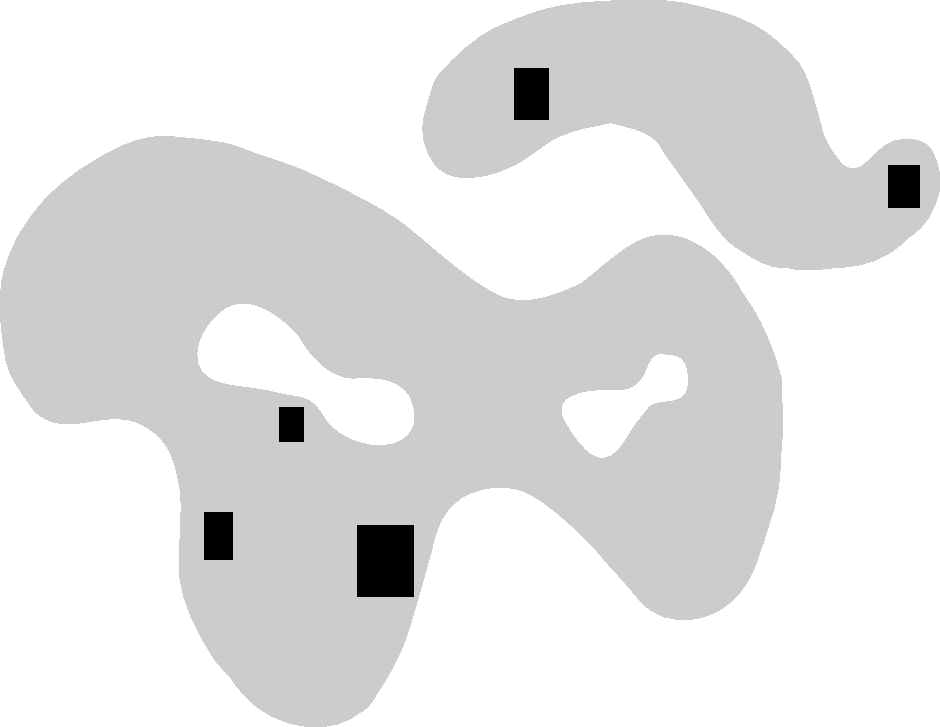
\includegraphics[width=.75\linewidth]{./pics/Fig1-1.pdf}
    \caption{}
    \label{Fig 1-1}
\end{figure}

The reader should supply the proof that a closed rectangle in
$\F{R}^n$ is indeed a closed set.

If $A\subset \F{R}^n$ and $x\in \F{R}^n$, then one of three possibilities must
hold (\figref{Fig 1-2}):
\begin{enumerate}[label={\upshape(\arabic*)}]
    \item There is an open rectangle $B$ such that $x\in B\subset A$
    \item There is an open rectangle $B$ such that $x \in B \subset C \subset \F{R}^n-A$.
    \item If $B$ is any open rectangle with $x\in B$, then $B$ contains points of both $A$ and $\F{R}^n-A$
\end{enumerate}

\begin{figure}[!htb]
    \centering
    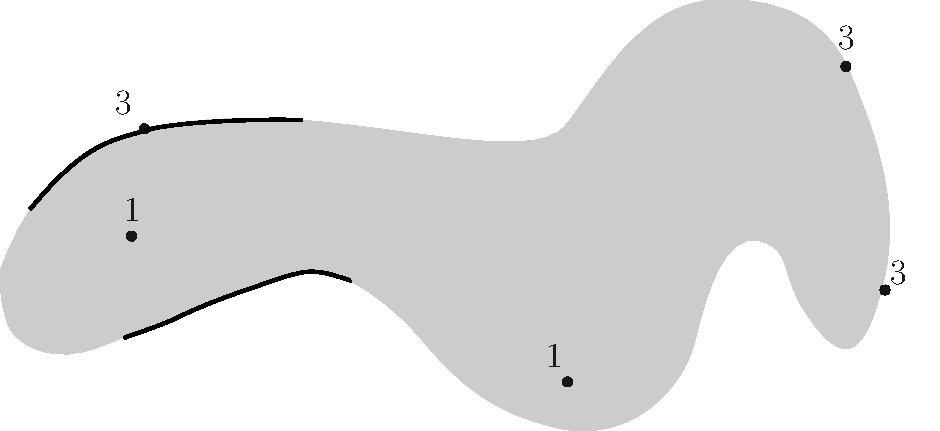
\includegraphics[width=.75\linewidth]{./pics/Fig1-2.pdf}
    \caption{}
    \label{Fig 1-2}
\end{figure}

Those points satisfying (1) constitute the \textbf{interior} of $A$, those
satisfying (2) the \textbf{exterior} of $A$, and those satisfying (3) the
\textbf{boundary} of $A$. Problems 1-16 to 1-18 show that these terms
may sometimes have unexpected meanings.

It is not hard to see that the interior of any set $A$ is open,
and the same is true for the exterior of $A$, which is, in fact, the
interior of $\F{R}^n-A$. Thus (Problem 1-14) their union is open,
and what remains, the boundary, must be closed.

A collection \C{O} of open sets is an \textbf{open cover} of $A$ 
(or, briefly,\textbf{covers} $A$) if every point $x \in A$ is 
in some open set in the collection \C{O}.
For example, if \C{O} is the collection of all open
intervals $(a, a + 1)$ for $a\in R$, then \C{O} is a cover of $\F{R}$.
Clearly no finite number of the open sets in \C{O} will cover $\F{R}$ or, 
for that matter, any unbounded subset of $\F{R}$.A similar situation can
also occur for bounded sets. 
If \C{O} is the collection of all open
intefvals $(1/n, 1-1/n)$ for all integers $n > 1$, then \C{O} is an
open cover of $(0,1)$, but again no finite collection of sets in
\C{O} will cover $(0,1)$.Although this phenomenon may not appear
particularly scandalous, sets for which this state of affairs
cannot occur are of such importance that they have received a
special designation: a set A is called \textbf{compact} if every open
cover \C{O} contains a finite subcollection of open sets which
also covers $A$.

A set with only finitely many points is obviously compact
and so is the infinite set $A$ which contains 0 and the numbers
$1/n$ for all integers $n$ (reason: if \C{O} is a cover, then $0 \in U$ for
some open set $U$ in \C{O}; there are only finitely many other points
of $A$ not in $U$, each requiring at most one more open set).

Recognizing compact sets is greatly simplified by the following 
results, of which only the first has any depth (i.e., uses any
facts about the real numbers).

\begin{theorem}[Heine-Borel]
    The closed interval $[a,b]$ is compact.
\end{theorem}

\begin{proof}
    If \C{O} is an open cover of $[a,b]$, let 
    $A = \{x:a\le x\le b\text{ and } [a, x]$ is covered by some finite number of open sets in \C{O}\}.
    \begin{figure}[!htb]
        \centering
        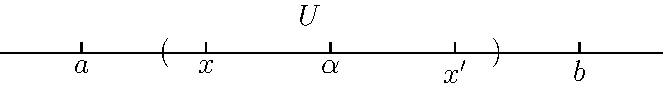
\includegraphics[width=.75\linewidth]{./pics/Fig1-3.pdf}
        \caption{}
        \label{Fig 1-3}
    \end{figure}

    Note that $a\in A$ and that $A$ is clearly bounded above (by b).
    We would like to show that $b\in A$. This is done by proving two things about $\alpha =$ least 
    upper bound of $A$; namely, (1) $a\in A$ and (2) $b=\alpha$.

    Since \C{O} is a cover, $\alpha \in U$ for some $U$ in \C{O}. Then all points in some interval 
    to the left of $\alpha$ are also in $U$(see \figref{Fig 1-3}). Since $\alpha$ is the least upper bound 
    of $A$, there is an $x$ in this interval such that $x\in A$. Thus $[a, x]$ is covered by some 
    finite number of open sets of $\C{O}$, while $[x, \alpha]$ is covered by the single set $U$. 
    Hence $[a, \alpha]$ is covered by a finite number of open sets of \C{O}, and $\alpha \in A$.
    This proves (1).

    To prove that (2) is true, suppose instead that $\alpha < b$.
    Then there is a point $x'$ between $\alpha$ and $b$ such that $[\alpha,x'] \subset U$.
    Since $\alpha\in A$, the interval $[\alpha,a]$ is covered by finitely many
    open sets of \C{O}, while $[\alpha, x']$ is covered by $U$.Hence $x' \in A$,
    contradicting the fact that $\alpha$ is an upper bound of $A$.
\end{proof}

If $B\subset \F{R}^m$ is compact and $x \in \F{R}^n$, it is easy to see that
$\{x\} \times B \subset \F{R}^{m+n}$ is compact.However, a much stronger assertion can be made.
\begin{theorem}
    If $B$ is compact and \C{O} is an open cover of
    $\{x\} \times B$, then there is an open set $U \subset \F{R}^n$ containing $x$ such
    that $U \times B$ is covered by a finite number of sets in \C{O}.
\end{theorem}

\begin{proof}
    Since $\{x\} \times B$ is compact, we can assume at the
    outset that \C{O} is finite, and we need only find the open set $U$
    such that $U \times B$ is covered by \C{O}.

    \begin{figure}[t]
        \centering
        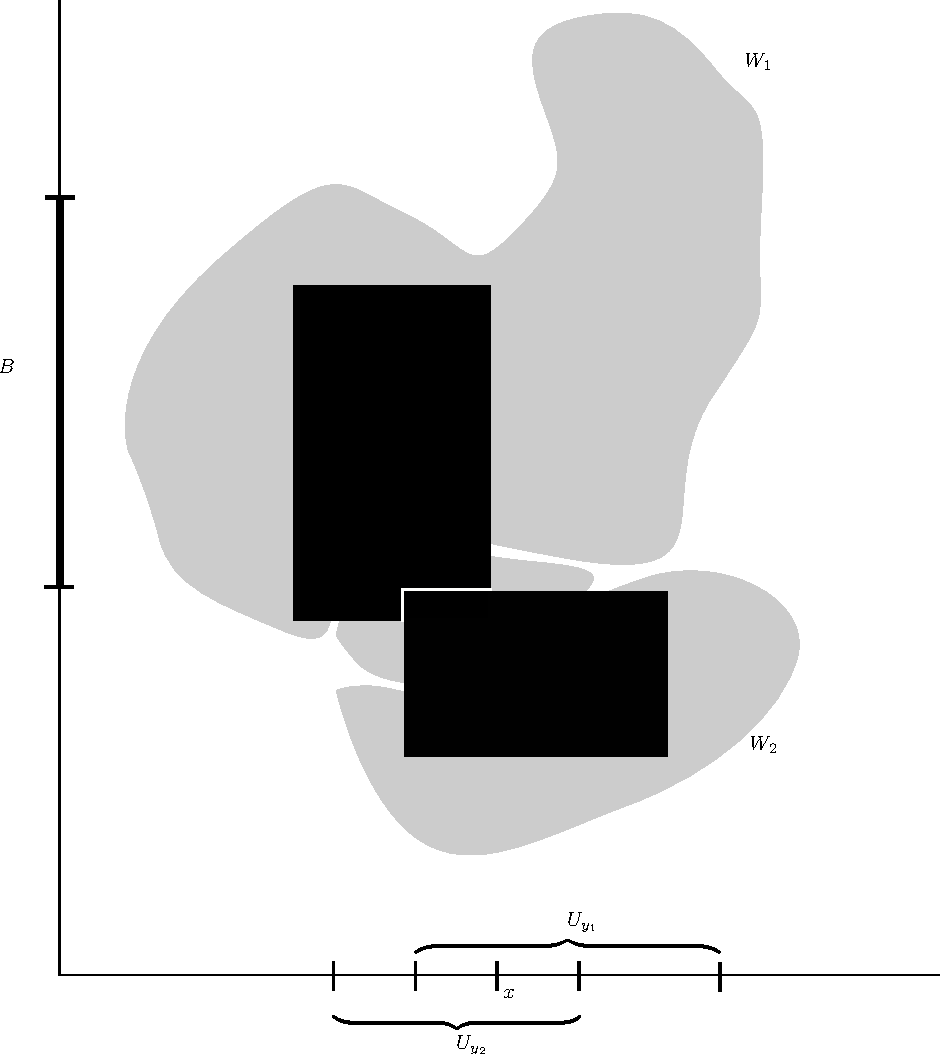
\includegraphics[width=.75\linewidth]{./pics/Fig1-4.pdf}
        \caption{}
        \label{Fig 1-4}
    \end{figure}

    For each $y\in B$ the point $(x, y)$ is in some open set $W$ in \C{O}.
    Since $W$ is open, we have $(x, y) \in U_y\times V_y\subset W$ for some 
    open rectangle $U_y\times V_y$. The sets $V_y$ cover the compact set $B$,
    so a finite  number $V_{y_1},\cdots, V_{y_k}$ also cover $B$. Let 
    $U = U_{y_1}\cap\cdots\cap U_{y_k}$, Then if $(x', y') \in U\times B$, 
    we have $y'\in V_{y_i}$ for some $i$ (\figref{Fig 1-4}), and certainly $x'\in U_{y_1}$.
    Hence $(x', y')\in U_{y_i}\times V_{y_i}$, which is contained in some $W$ in \C{O}.
\end{proof}

\begin{corollary}
    If $A\subset \F{R}^n$ and $B\subset \F{R}^n$ are compact, then 
    $A\times B\subset \F{R}^{m+n}$ is compact. 
\end{corollary}

\begin{proof}
    If \C{O} us an open cover of $A\times B$, then \C{O} covers $\{x\}\times B$ 
    for each $x\in A$. By Thereom 1-4 there is an open set $U_x$ containing 
    $x$ such that $U_x\times B$ is covered by finitely many sets in \C{O}.
    Since $A$ is compact, a finite number of $U_{x_1}, \cdots, U_{x_n}$ of 
    the $U_x$ cover $A$. Since finitely many sets in $\C{O}$ cover each $U_{x_i}\times B$,
    finite many cover all of $A\times B$. 
\end{proof}

\begin{corollary}
    $A_1\times \cdots\times A_k$ is compact if each $A_i$ is.
    In particular, a closed rectangle in $\F{R}^k$ is compact. 
\end{corollary}

\begin{corollary}
    A closed bounded subset of $\F{R}^n$ is compact. (The converse is also true (Problem 1-20).)
\end{corollary}

\begin{proof}
    If $A \subset \F{R}^n$ is closed and bounded, then $A \subset B$ for
    some closed rectangle $B$. If \C{O} is an open cover of $A$, then \C{O}
    together with $\F{R}^n-A$ is an open cover of $B$. Hence a finite
    number $U_1, \cdots , U_n$ of sets in \C{O}, together 
    with $\F{R}^n-A$ perhaps, cover $B$. Then $U_1, \cdots, U_n$ cover $A$. 
\end{proof}

\begin{problems}
    \problem[*]{Prove that the union of any (even infinite) number
        of open sets is open. Prove that the intersection of two (and hence
        of finitely many) open sets is open. Give a counterexample for
        infinitely many open sets.}
    \problem{Prove that $\{x\in \F{R}^n: |x-a|< r\}$ is open(see also Problem 1-27).}
    \problem{Find the interior, exterior, and boundary of the sets
        \begin{align*}
            & \{x\in \F{R}^n: |x|< 1\} \\
            & \{x\in \F{R}^n: |x|= r\} \\
            & \{x\in \F{R}^n: \text{each}~ x^i \text{ is rational}\}.
        \end{align*}
    }
    \problem{Construct a set $A \subset [0,1] \times [0,1]$ such that $A$ contains at most
        one point on each horizontal and each vertical line but boundary
        $A = [0,1] \times [0,1]$.\textit{Hint:} It suffices to ensure that A contains
        points in each quarter of the square $[0,1] \times [0,1]$ and also in each
        sixteenth, etc.}
    \problem[*]{If $A \subset [0,1]$ is the union of open intervals $(a_i,b_i)$ such that each
        rational number in $(0,1)$ is contained in some $(a_i,b_i)$, show that
        boundary $A = [0,1] - A$.}
    \problem{If $A$ is a closed set that contains every rational number $r \in [0,1]$,
        show that $[0,1] \subset A$.}
    \problem{Prove the converse of Corollary 1-7: A compact subset of $\F{R}^n$ is closed and 
        bounded (see also Problem 1-28)}
    \problem{
        \begin{enumerate}[label={\upshape(\alph*)}]
            \item If $A$ is closed and $x\notin A$, prove that there is a number $d>0$ such that 
                $|x-y| \ge d$ for all $y\in A$.
            \item If $A$ is closed, $B$ is compact,and  $A\cap B = \ns$, prove that 
                there is $d>0$ such that $|y-x|\ge d$ for all $y\in A$ and $x\in B$.\textit{Hint:}
                For each $b\in B$ find an open set $U$ containing $b$ such that this relation holds for 
                $x\in U\cap B$
            \item Give a counterexample in $\F{R}^2$ if $A$ an $B$ are closed but neither is compact. 
        \end{enumerate}
    }
    \problem[*]{If $U$ is open and $C\subset U$ is compact, show that there is a compact set $D$ such that 
        $C\subset$ interior $D$ and $D\subset U$.}
\end{problems}




